\documentclass[11pt,a4paper]{article}
\usepackage[T1]{fontenc}\usepackage[utf8]{inputenc}
\usepackage{lmodern,microtype,amsmath,amssymb,amsthm,mathtools}
\usepackage{booktabs,longtable,array,enumitem,xcolor,geometry,fancyhdr,hyperref,graphicx}
\geometry{margin=22mm}
\hypersetup{colorlinks=true,linkcolor=blue!55!black,urlcolor=blue,citecolor=blue!55!black,
 pdftitle={FIN ST1812--ST1901: Direct Gauge-Covariant Dirichlet Action, Topology, Refinement and Spectral-Triple Obstructions},
 pdfauthor={Krzysztof Żuchowski}}
\pagestyle{fancy}\fancyhf{}\fancyhead[L]{FIN ST1812--ST1901}\fancyhead[R]{Release 11.04}\fancyfoot[C]{\thepage}\setlength{\headheight}{14pt}
\newtheorem{theorem}{Theorem}\newcommand{\status}[1]{\textsf{[#1]}}

\begin{document}
\begin{titlepage}\centering\vspace*{14mm}
{\Huge\bfseries FIN ST1812--ST1901\par}\vspace{4mm}
{\LARGE Direct Gauge-Covariant Dirichlet Action,\par}\vspace{2mm}
{\LARGE Topology, Refinement and Spectral-Triple Obstructions\par}\vspace{12mm}
{\Large Krzysztof \.Zuchowski\par}
{\normalsize Independent Researcher --- Fractal Information Theory Project\par}
{\normalsize ORCID: 0009-0002-0909-3613\par}\vspace{9mm}
{\large Six adaptive research rounds --- 90 programmes\par}
{\large Release 11.04 --- 1 September 2026\par}
\vfill
\begin{minipage}{.87\textwidth}\small
This report follows the Release 11.03 falsification of the APD--moment--
$L_{\rm total}$ route.  It attempts a different construction directly from the
strict Dirichlet form: a first-order weighted differential and a locally
gauge-covariant lattice matter action.  The construction is then immediately
tested for uniqueness, curvature, refinement, continuum, chirality, fermions
and gravity.
\end{minipage}\vfill
{\small English mathematical and critical research report.}
\end{titlepage}

\begin{abstract}
ST1812--ST1901 investigate whether the strict FIN Dirichlet form can produce a
gauge-covariant action without the previously falsified APD and three-moment
routes.  The answer is conditionally positive for finite matter dynamics and
negative for unique physical gauge geometry.

Because every strict off-diagonal weight is positive, the current support is
the complete graph $K_{12}$.  Choosing one orientation per edge defines a
weighted incidence operator $d_W$ with
\[
A=d_W^*d_W.
\]
Introducing $U(1)$ link phases gives the covariant difference
\[
(d_U\psi)_{ij}=\sqrt{w_{ij}}(\psi_i-U_{ij}\psi_j)
\]
and the action
\[
S_{\rm matter}[\psi,U]
=\frac12\sum_{i<j}w_{ij}|\psi_i-U_{ij}\psi_j|^2
+\sum_iV(|\psi_i|^2).
\]
It is globally regular, positive and exactly invariant under local vertex
phases.  Literal variation gives one coherent covariant Euler equation, and
$U=1$ recovers the strict $A$.  Thus a minimal conditional gauge-matter repair
exists directly from the Dirichlet form.

Immediate falsification shows why this is not yet strict physics.  The same
weights admit $U(1)$ with every integer charge, $Z_N$, $SU(2)$, $U(k)$ and real
non-gauge models.  Complexification, gauge group, representation, connection
state and radial-potential coefficients are not selected by $A$.  First-order
factorizations are nonunique unless an edge-locality axiom is added.

Gauge dynamics is more obstructed.  The $K_{12}$ one-skeleton has 66 edges and
cycle rank 55.  Without 2-cells it has 55 independent holonomies and no local
curvature action.  There are 220 triangle cliques; their boundary map has rank
55, and the full clique complex is the contractible 11-simplex.  Adding every
triangle removes first homology but still leaves arbitrary face areas and
Wilson coefficients.  Thresholding to the nearest-neighbour $C_{12}$ creates
$H^1$ of dimension one only by discarding 54 nonzero strict edges.  The
support graph has diameter one, so it does not supply extended locality or a
3+1-dimensional Maxwell limit.

The exact refinement
$A_{24}=A_{12}\otimes I_2+I_{12}\otimes B_q$ transports the normalized
fiber-constant matter action, but grows the cycle rank from 55 to 121, adds
relative fiber phases, and leaves $q$, lengths, face areas and scaling laws
free.  It does not select a continuum.

A first-order fermionic test gives another split result.  No nontrivial
vertex-diagonal grading anticommutes with a full-support vertex Dirac operator:
triangles make the sign equations inconsistent.  Doubling vertices and edges
produces an even incidence Dirac operator with square containing $A$, but the
78-dimensional space has 56 zero modes (one constant vertex mode and 55 cycle
modes).  Its index equals the graph Euler characteristic $12-66=-54$, not a
derived particle-generation index.  Edge-algebra representation, real
structure, first-order condition, fermion content, cutoff scale and gravity
remain additional data.

The direct gauge action therefore passes important conditional subrows of the
source--action gate but zero complete strict rows.  The highest-value next
theorem is now sharply identified: derive or refute an automorphism-natural,
refinement-functorial weighted 2-complex and face measure from FIN data.  Such
an object is required before a strict gauge kinetic action, locality or
continuum physics can be claimed.
\end{abstract}

\tableofcontents\newpage

\section{Starting point after Release 11.03}

Release 11.03 established that the APD quotient, three moment features and the
current mixed-lineage $L_{\rm total}$ do not derive unique physical dynamics.
The surviving unavoidable variational object is
\[
S_A[f]=\frac12f^TAf.
\]
The present cycle asks whether the first-order square root of this form can
supply a better source action without fitting effective couplings.

The test is intentionally stronger than constructing a gauge-looking formula.
Every positive construction is immediately checked for:
\begin{enumerate}
\item strict source and uniqueness;
\item a gauge kinetic/curvature term;
\item refinement naturality and continuum scaling;
\item chiral fermionic and gravitational content;
\item compatibility with the seven-row source--action gate.
\end{enumerate}

\section{Round I: ST1812--ST1826 --- direct gauge-covariant action}

Orient every unordered pair once and define
\[
(d_Wf)_{ij}=\sqrt{w_{ij}}(f_i-f_j),qquad i<j.
\]
The edge-sum identity gives
\[
d_W^*d_W=A
\]
to numerical residual below $10^{-15}$ in the independent reconstruction.
Orientation reversal changes a row convention but not the norm.

For unit link phases $U_{ij}$ with $U_{ji}=\overline{U}_{ij}$ define
\[
(d_U\psi)_{ij}=\sqrt{w_{ij}}(\psi_i-U_{ij}\psi_j).
\]
Under
\[
\psi_i\mapsto g_i\psi_i,qquad
U_{ij}\mapsto g_iU_{ij}g_j^{-1},qquad g_i\in U(1),
\]
one has
\[
(d_{U'}\psi')_{ij}=g_i(d_U\psi)_{ij}.
\]
Therefore
\[
S_{\rm matter}=\frac12\|d_U\psi\|^2+\sum_iV(|\psi_i|^2)
\]
is exactly gauge invariant.  The covariant Laplacian
$A_U=d_U^*d_U$ is Hermitian positive semidefinite, and $U=1$ gives $A$.

Literal variation yields
\[
A_U\psi+V'(|\psi|^2)\psi=J.
\]
A random finite gauge transformation reproduced the action exactly in double
precision.  The configuration space $U(1)^{66}\times\mathbb C^{12}$ contains
no APD poles.

\begin{theorem}[conditional minimal gauge-matter completion]
After choosing a complex scalar, local $U(1)$ symmetry with unit charge, one
link per nonzero edge and radial potential, the weighted covariant difference
is a globally regular positive gauge-invariant completion of the strict
Dirichlet matter action.
\end{theorem}

The theorem does not contain gauge-field kinetic dynamics.

\section{Round II: ST1827--ST1841 --- uniqueness falsification}

The flat connection $U=1$ erases the group and charge information.  The same
Dirichlet weights support:
\begin{itemize}
\item $U(1)$ with every integer charge via $U_{ij}^q$;
\item discrete $Z_N$ link fields;
\item non-Abelian $SU(2)$ or $U(k)$ links in any unitary representation;
\item the original real classical/Markov theory without complex phase.
\end{itemize}
All reduce to the same $A$ at the identity connection.

The factorization itself has edge-Hilbert freedom:
\[
A=d_W^*d_W=(Od_W)^*(Od_W)
\]
for every edge-space unitary/orthogonal $O$.  Requiring one edge degree of
freedom per nonzero pair and support locality reduces this to harmless
orientation/phase conventions, but that requirement is an additional
calculus axiom.

Because all off-diagonal entries are nonzero, the support graph $K_{12}$ is
canonical at the support level.  However, $A$ contains no nontrivial link
phases, holonomy state, charge, group or scalar representation.  Gauge
covariance constrains the form of radial potentials but not their coefficients.

Thus the direct action is the minimal repair \emph{conditional} on a chosen
gauge principle; it is not a unique physical consequence of FIN.

\section{Round III: ST1842--ST1856 --- curvature and topology}

The complete support has
\[
V=12,qquad E=66,qquad b_1=E-V+1=55.
\]
An edge connection modulo vertex gauge therefore has 55 independent cycle
holonomies if no faces are specified.

There are
\[
\binom{12}{3}=220
\]
triangle cliques.  Exact integer linear algebra gives rank 55 for the
triangle-to-edge boundary matrix.  Attaching all triangles kills the
one-skeleton $H^1$; attaching all higher cliques gives the full 11-simplex,
which is contractible.

A Wilson family can be written as
\[
S_g=\sum_f\kappa_f(1-\operatorname{Re}U_f),
\]
but $A$ does not select the face set, face orientation, area or coefficients
$\kappa_f$.  Products, geometric means, minima and external areas all define
different positive face measures.

Thresholding cyclic distance gives another nonunique topology.  Keeping only
distance one yields $C_{12}$ with 12 edges and $b_1=1$, but discards 54
strict nonzero edges.  Increasing the retained distance changes the edge and
cycle counts at every step.  No threshold is selected by nonzero support.

\begin{theorem}[support-to-curvature nonuniqueness]
The strict weighted support determines neither a unique 2-complex nor a unique
local gauge kinetic action.  The full support has graph diameter one and does
not by itself define extended locality or a 3+1-dimensional Maxwell limit.
\end{theorem}

\section{Round IV: ST1857--ST1871 --- refinement}

For $q>0$, the exact two-fiber refinement has
\[
A_{24}=A_{12}\otimes I_2+I_{12}\otimes B_q,
\]
with 24 vertices, 144 edges and cycle rank
\[
144-24+1=121.
\]
Its weighted incidence factorization reproduces $A_{24}$ to machine precision.

Copy a base connection to both fibers, set the fiber connection flat, and use
the normalized constant fiber vector $u_+=(1,1)/\sqrt2$.  Then
\[
(\psi\otimes u_+)^*A_{24}(\psi\otimes u_+)=\psi^*A_{12}\psi.
\]
Thus the matter action transports exactly.

The full fine gauge group has 24 local phases rather than 12.  Twelve relative
fiber phases and twelve fiber link variables are invisible to the coarse
factorized subgroup.  The rate $q$ remains free.  Each further binary
refinement introduces at least one new rate and relative connection layer
unless a consistency law is supplied.

The refined support is $K_{12}\square K_2$, with degree 12 and diameter two.
It remains highly nonlocal rather than approaching an extended continuum.
No scaling law for $q$, edge lengths, face areas, effective dimension or causal
speed is exported.

The positive conclusion is exact refinement transport of matter dynamics.
The negative conclusion is that refinement does not select locality, topology,
dimension or continuum gauge physics.

\section{Round V: ST1872--ST1886 --- Dirac, chirality and gravity}

A naive symmetric vertex operator built from $\sqrt{w_{ij}}$ does not square
to $A$.  More importantly, suppose a vertex-diagonal grading
$\Gamma=\operatorname{diag}(\gamma_i)$ with $\gamma_i=\pm1$ anticommutes with a
full-support vertex Dirac operator.  Every nonzero edge requires
$\gamma_j=-\gamma_i$.  A triangle then gives a contradiction.  Therefore no
nontrivial vertex-diagonal even grading exists on the complete support.

A standard first-order repair doubles vertices and edges:
\[
\mathcal D=
\begin{pmatrix}0&d_W^*\\d_W&0\end{pmatrix},qquad
\Gamma=\begin{pmatrix}I_{12}&0\\0&-I_{66}\end{pmatrix}.
\]
Then $\{\Gamma,\mathcal D\}=0$ and
\[
\mathcal D^2=operatorname{diag}(A,d_Wd_W^*).
\]
The 78-dimensional operator has 22 nonzero modes and 56 zero modes: one
constant vertex mode and 55 edge-cycle modes.  Its incidence index is
\[
1-55=12-66=-54,
\]
the graph Euler characteristic, not a derived physical generation count.

This even complex is not yet a real spectral triple.  A vertex-function
algebra has no unique action on unoriented edges: source, target, average and
doubled-oriented representations differ.  Reality, first-order condition and
orientation cycle are missing.  Inner fluctuations require those choices.

A spectral action further needs a cutoff function, dimensional cutoff,
fermionic representation and gauge kinetic normalization.  The incidence
Dirac does not supply a 3+1 spin structure, Lorentzian signature, metric tensor
or diffeomorphism/gravity action.

\section{Round VI: ST1887--ST1901 --- final gate and verdict}

\begin{longtable}{@{}p{.35\textwidth}p{.20\textwidth}p{.35\textwidth}@{}}
\toprule
Object & Status & Boundary \\
\midrule\endhead
$A=d_W^*d_W$ & \status{Proven} & finite weighted graph \\
local $U(1)$ matter action & \status{Proven conditional} & chosen complex field/group/links \\
gauge group, charge and connection & \status{Not sourced} & many exact alternatives \\
canonical gauge kinetic action & \status{Refuted from support alone} & face/area ambiguity \\
coarse refinement transport & \status{Proven} & factorized connection/constant fiber \\
continuum dimension/locality & \status{Not derived} & free scaling/moduli \\
even incidence Dirac & \status{Constructed} & 56 zero modes \\
real/chiral SM spectral triple & \status{Not derived} & algebra/reality/representation missing \\
gravity/physical gauge theory & \status{Not established} & scale, topology, platform absent \\
\bottomrule
\end{longtable}

The updated strict gauge-source gate contains seven rows:
\begin{enumerate}[label=H\arabic*.]
\item strict state-category/gauge-group/charge source;
\item strict connection/holonomy source;
\item canonical 2-complex, face measure and gauge kinetic action;
\item refinement scaling to local continuum dimension and causality;
\item real even spectral triple with chiral fermion representation;
\item dimensional action and nonabsorbable prediction;
\item OA platform and independent record.
\end{enumerate}
The direct action makes conditional progress on regularity, gauge covariance
and literal variation, but zero rows are complete in the strict sense.

\begin{figure}[ht]
\centering
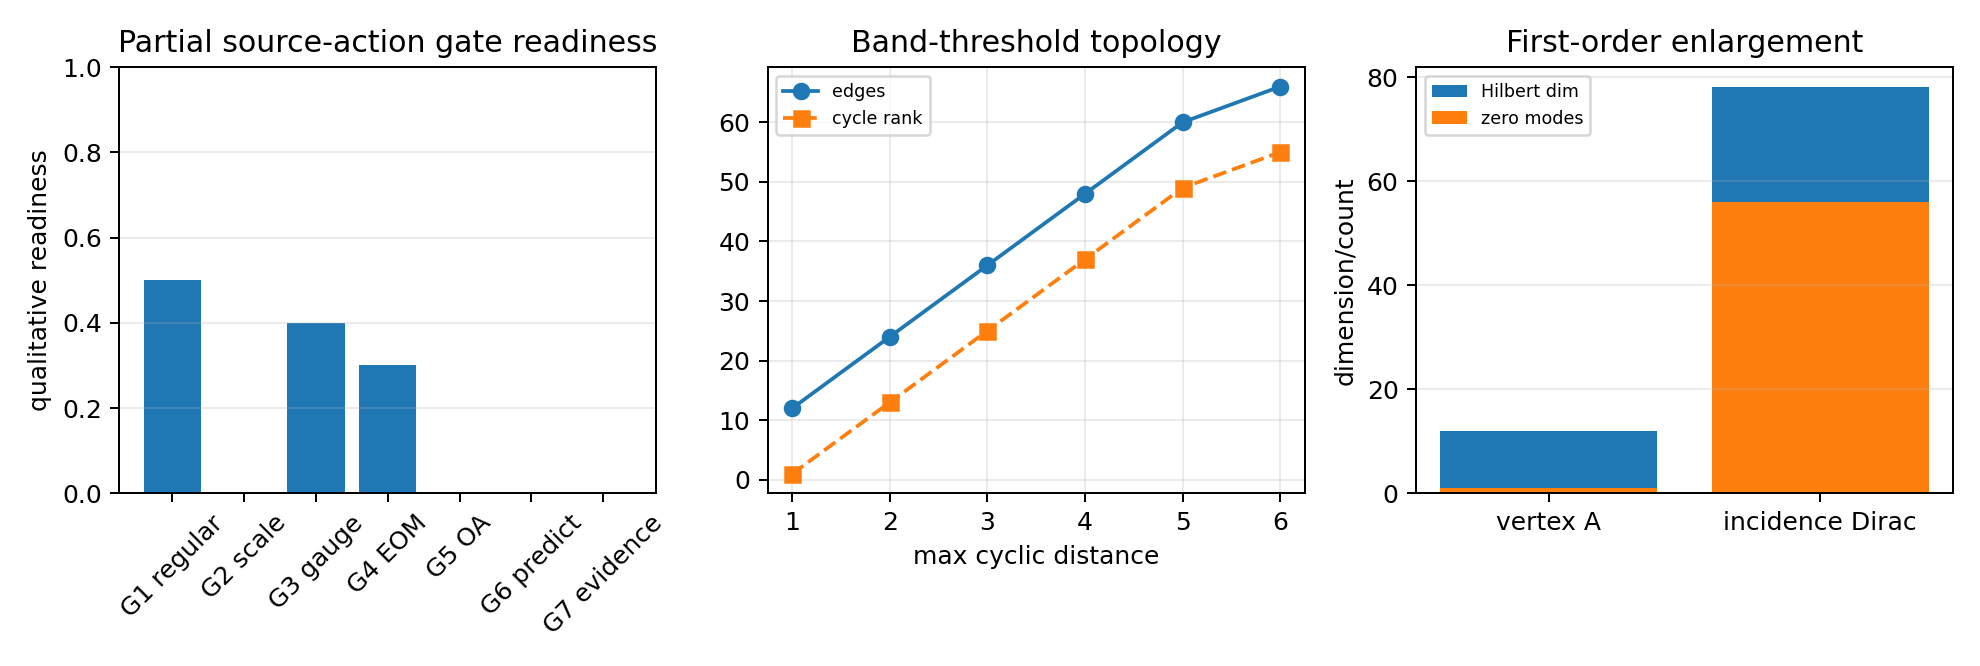
\includegraphics[width=.98\textwidth]{FIN_ST1812_ST1901_Figures/gauge_source_action_audit.png}
\caption{Left: qualitative partial readiness of the prior source--action gate.
Centre: topology changes under distance-band thresholding.  Right: the
first-order incidence construction enlarges the state space and creates 56
zero modes.}
\end{figure}

\section{Most important result}

The most important result is the constructive/negative pair:
\[
\boxed{
\text{strict Dirichlet data admits a clean conditional gauge-matter action,}
}
\]
but
\[
\boxed{
\text{it does not select gauge group, curvature complex, continuum or chiral
physics.}
}
\]

This is more informative than the earlier $L_{\rm total}$ scaffold.  Gauge
invariance and one-action EOM can be repaired without APD or moment fitting,
but the repair exposes exactly which new objects are still absent.

\section{Highest-value next theorem}

The single most decisive next target is:
\begin{quote}
\emph{derive or refute an automorphism-natural, refinement-functorial map from
strict FIN data to an oriented weighted 2-complex with positive face measure,
whose Wilson or spectral gauge action has a controlled local continuum limit.}
\end{quote}

It should be falsified in this order:
\begin{enumerate}
\item automorphism naturality;
\item independence of arbitrary thresholds;
\item refinement functoriality;
\item local dimension and causal scaling;
\item positive face weights;
\item continuum Maxwell normalization.
\end{enumerate}

If no such functor exists from the full strict/refinement data, the gauge-field
route from FIN is blocked without new physics by assumption.  If it does
exist, it would close the most important gap left by this cycle and provide a
real input for a spectral/source action.

\section{Route ranking}

\begin{longtable}{@{}p{.53\textwidth}p{.18\textwidth}p{.18\textwidth}@{}}
\toprule
Route & Rigorous-success estimate & Physics decision power \\
\midrule\endhead
derive canonical 2-complex/face measure from refinement & 0.28 & 1.00 \\
publish conditional $U(1)$ Dirichlet lattice matter model & 0.80 & 0.45 \\
complete real even spectral triple from incidence complex & 0.30 & 0.75 \\
continue APD/moment $L_{\rm total}$ repair & 0.01 & 0.50 \\
OA laboratory test of frozen channels & 0.45 & 0.55 \\
\bottomrule
\end{longtable}

These estimates are strategic judgments, not empirical probabilities.

\section{Final interpretation}

\begin{quote}
The direct first-order Dirichlet construction is currently the most promising
mathematical bridge from FIN toward gauge theory because it is globally
regular, positive, exactly gauge covariant and variationally coherent.  It is
still conditional rather than strict: the group, charge, connection state,
2-complex, face weights, scale, fermions and platform are not derived.  FIN
therefore remains a finite Dirichlet--Markov--spectral information geometry
with a viable conditional lattice gauge-matter extension, not a fundamental
physical theory.
\end{quote}

\appendix
\section{Six-round ledger}
\begin{longtable}{@{}p{.18\textwidth}p{.34\textwidth}p{.38\textwidth}@{}}
\toprule
Range & Target & Verdict \\
\midrule\endhead
ST1812--ST1826 & covariant Dirichlet matter action & exact conditional construction \\
ST1827--ST1841 & uniqueness & group/charge/calculus nonuniqueness \\
ST1842--ST1856 & curvature topology & no canonical 2-complex/Maxwell action \\
ST1857--ST1871 & refinement & matter transports; continuum not selected \\
ST1872--ST1886 & Dirac/fermions/gravity & even complex, large zero sector, physics open \\
ST1887--ST1901 & synthesis & updated seven-row gauge-source gate \\
\bottomrule
\end{longtable}

\section{Reproducibility}
The authoritative result sets run from
\path{FIN_ST1812_ST1826_Results.json} through
\path{FIN_ST1887_ST1901_Results.json}.  Each contains fifteen programmes and
packet SHA-256 references.  The combined test
\path{test_fin_st1812_st1901.py} verifies all ninety packets, gauge invariance,
topological ranks, refinement factorization, grading/zero modes, updated gate,
figure and nonpromotion boundaries.

\section{Nonclaims}
This report does not derive the gauge group, charge, connection state, Wilson
face action, continuum spacetime, chirality, fermion generations, gravity,
physical units, state ontology, platform or evidence.  It does not complete
legacy role transfer, QW-2191, Standard Model, $L_{\rm total}$ or Theory of
Everything.  All future FIN PDFs remain English.

\begin{thebibliography}{9}
\bibitem{rothe} H. J. Rothe, \emph{Lattice Gauge Theories}, World Scientific.
\bibitem{connes} A. Connes and M. Marcolli, \emph{Noncommutative Geometry, Quantum Fields and Motives}, AMS.
\bibitem{chung} F. Chung, \emph{Spectral Graph Theory}, AMS.
\end{thebibliography}
\end{document}
